\documentclass[10pt]{exam}
\usepackage[phy]{template-for-exam}
\usepackage{tikz, multicol}

\title{Simple Harmonic \#1}
\author{Rohrbach}
\date{\today}

\begin{document}
\maketitle

\begin{questions}
\question
  What are the two things that affect the period of a pendulum?
  \vs

\question
  Why does amplitude \emph{not} affect the period of a pendulum?
  \vs[2]

\question
  Why does mass \emph{not} affect the period of a pendulum?
  \vs[2]

\question
  Pendulum A and pendulum B are identical, except that pendulum A has twice as much amplitude.

  \begin{multicols}{2}

    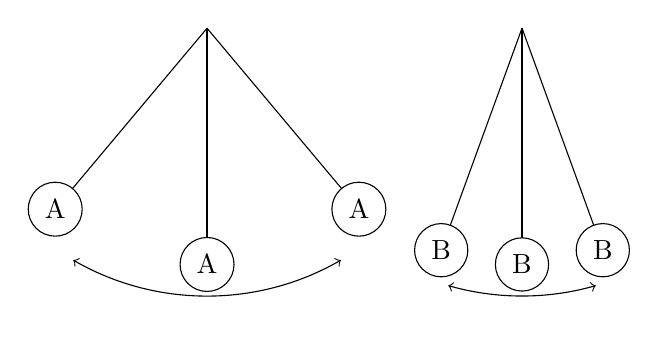
\begin{tikzpicture}[
      bob/.style={
        draw=black, fill=white, circle, radius=0.3
      }
      ]

        \begin{scope}
          \draw[<->] (-120:3.4) arc (-120:-60:3.4);
          \draw (-130:3) node[bob] {A} -- (0,0);
          \draw (-90:3) node[bob] {A} -- (0,0);
          \draw (-50:3) node[bob] {A} -- (0,0);  
        \end{scope}

        \begin{scope}[shift={(4,0)}]
          \draw[<->] (-106:3.4) arc (-106:-74:3.4);
          \draw (-110:3) node[bob] {B} -- (0,0);
          \draw (-90:3) node[bob] {B} -- (0,0);
          \draw (-70:3) node[bob] {B} -- (0,0);  
        \end{scope}
  

  
    \end{tikzpicture}
  
    \columnbreak

    \begin{parts}
      \part 
        Which pendulum has the longer period?  How do you know?
        \vspace{6em}
      \part 
        Which pendulum has the faster top speed?  How do you know?
        \vspace{6em}
    \end{parts}
  \end{multicols}





\question
  What are the four equations you will need to memorize for this unit?
  \vs[2]

\pagebreak

\question
  In order to capture video, a video camera takes 32 pictures per second.

  \begin{parts}
    \part 
      What is the frequency with which the camera takes pictures?
      \vs
    \part 
      What is the period?
      \vs
  \end{parts}


\question
  A flautist in the marching band makes 120 steps in one minute (60 seconds).

  \begin{parts}
    \part 
      What is the frequency with which the flautist takes step?
      \vs
    \part 
      What is the period?
      \vs
  \end{parts}


\question
  What is the (a) period and (b) frequency of a pendulum that has a mass of 0.25 kg and a length of 2 meters?
  \vs[3]

\question
  What is the length of a pendulum that has a period of 5.2 seconds?
  \vs[3]




\end{questions}

\end{document}